\allowdisplaybreaks[4]

為了驗證本研究模型在真實場景中的應用潛力，本研究開發了一套即時音訊深偽偵測系統。系統採用前後端分離（Decoupled Architecture）架構，以確保系統的擴充性與推論效率：
\begin{enumerate}
    \item{前端展示層 (Next.js)：}
    採用 Next.js 框架構建。利用其高效的路由管理與組件化開發優勢，實現響應式網頁介面。前端負責處理音訊錄製、檔案上傳與即時波形顯示，並透過 RESTful API 與後端進行異步通訊。
    \item{後端推論層 (FastAPI \& PyTorch)：}
    後端核心採用 FastAPI 框架，其異步處理能力能有效降低多模型併發推論時的延遲。模型推理部分則由 PyTorch 驅動，整合了本研究所介紹的三種深偽檢測模型 MFA-Conformer、W2V-AASIST、SpeechPrompt v2、TTS 模型 IndexTTS2，以及將語音轉錄成文本的 ASR 模型 Whisper。
    \item{快速部署環境 (Docker \& uv)：}
    為了應對深度學習環境中複雜的依賴關係（如特定版本的 CUDA、cuDNN、PyTorch 與 FastAPI 依賴庫），本系統全面採用 Docker 容器化技術，並利用 uv 快速安裝相應的依賴套件。
\end{enumerate}

\begin{figure}[H]
    \centering
    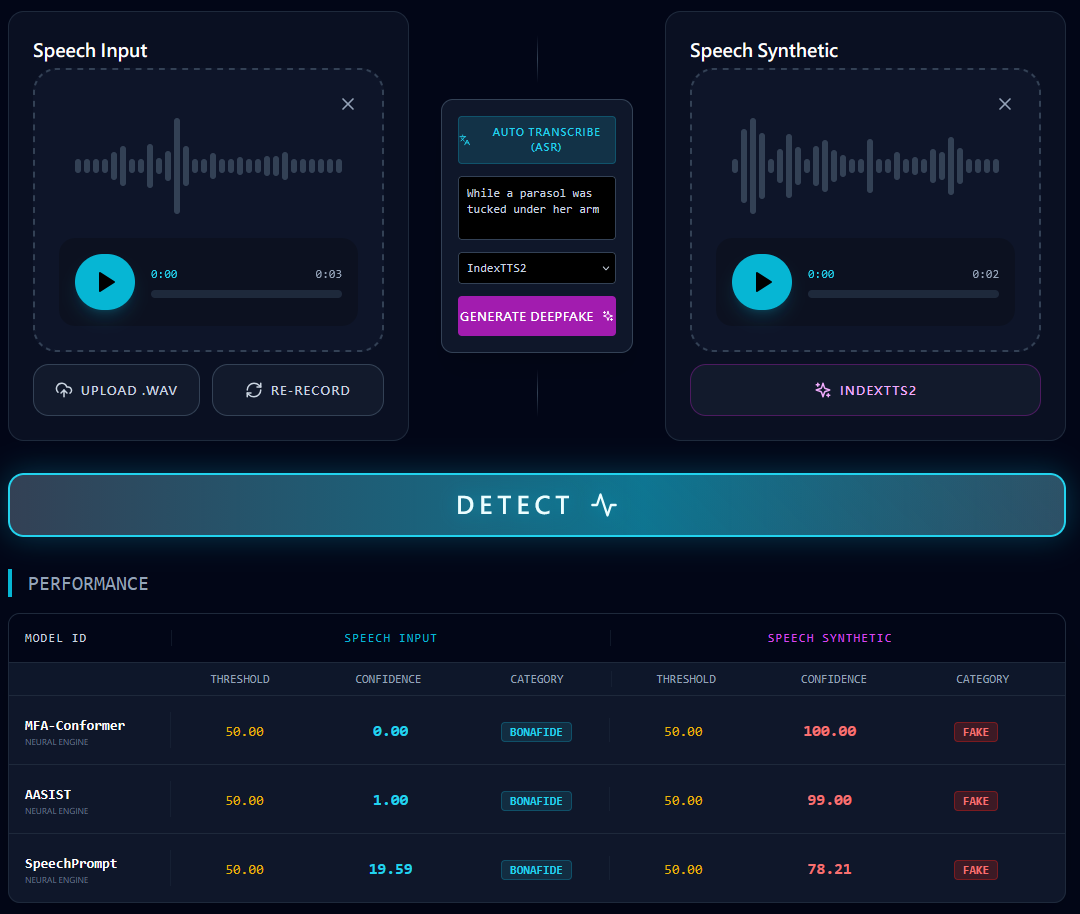
\includegraphics[width=1.0\textwidth]{images/adf3.png}
    \caption{前端應用網頁。左上區塊為語音輸入模組，右上區塊為語音生成模組，下半部為偵測結果展示區。}
    \label{fig:system_architecture}
\end{figure}

前端頁面如圖\ref{fig:system_architecture}
所示，包含語音輸入、語音生成、與偵測結果三大功能區塊。以下說明各區塊的功能與操作流程：

\section{語音輸入與文本來源}
系統提供兩個音訊來源管道，如圖\ref{fig:system_architecture}左上區塊。使用者可透過錄音按鈕進行即時採樣，亦可點擊上傳按鈕選擇本地音訊檔案。音訊載入後，文本來源可由兩種方式取得：其一為點擊 ASR 按鈕，利用 Whisper 模型自動轉錄語音；其二為於文本框內自行輸入或修改內容，以測試特定語句在深偽生成下的表現。
\section{音訊生成與偽造}
在取得參考音訊與文本後，使用者可於語音生成模組選擇 TTS 引擎（預設為 IndexTTS2.0），並點擊「Generate Deepfake」生成偽造語音。系統會參照原始音訊的音色特徵進行合成，並於右上「Speech Synthetic」區塊顯示波形與播放控制項，供使用者即時預覽生成品質。
\section{偵測核心與效能呈現}
當使用者點擊「Detect」按鈕後，系統會將「Speech Input」與「Speech Synthetic」中的語音同時送往後端模型進行推理。結果區域以列表方式呈現不同模型的判別數據，並支援真偽語音之對照分析與多模型交叉驗證。
\begin{enumerate}
     \item{模型標識 (Model ID)}
        列出參與評測的模型架構。
        \item{機率分佈 (Confidence Score)}
        顯示「真實 (Bonafide)」與「偽造 (Spoof)」的機率百分比。其數值由模型輸出之 Logits 經過 Softmax 轉換所得：
        \begin{equation}
        P_{i} = \frac{e^{z_i}}{\sum_{j \in \{B, S\}} e^{z_j}}
        \end{equation}
        其中 $z$ 為模型最後一層線性層輸出之原始分數 (Logits)，$i \in \{B, S\}$ 分別代表真音與偽造語音類別。
        
        \item{判定門檻 (Threshold)}
        門檻值 τ 為系統判定真偽的裁決基準。本平台允許針對不同模型設定獨立的門檻值，其設定依據各模型在開發集（Dev set）上取得等錯誤率（EER）時的決策點。若模型輸出之偽造機率 $P_S > \tau$（預設 $\tau = 0.5$），系統將判定為「Spoof」並以紅色高亮顯示；反之則判定為「Bonafide」。

\end{enumerate}

本系統之展示頁面已公開於 GitHub：\url{https://github.com/brant92good/ADF_website}，可透過 Docker 快速部署，供後續研究參考。
